% Options for packages loaded elsewhere
\PassOptionsToPackage{unicode}{hyperref}
\PassOptionsToPackage{hyphens}{url}
\PassOptionsToPackage{dvipsnames,svgnames,x11names}{xcolor}
%
\documentclass[
  12pt,
  letterpaper,
]{report}

\usepackage{amsmath,amssymb}
\usepackage{lmodern}
\usepackage{iftex}
\ifPDFTeX
  \usepackage[T1]{fontenc}
  \usepackage[utf8]{inputenc}
  \usepackage{textcomp} % provide euro and other symbols
\else % if luatex or xetex
  \usepackage{unicode-math}
  \defaultfontfeatures{Scale=MatchLowercase}
  \defaultfontfeatures[\rmfamily]{Ligatures=TeX,Scale=1}
  \setmainfont[]{Times New Roman}
\fi
% Use upquote if available, for straight quotes in verbatim environments
\IfFileExists{upquote.sty}{\usepackage{upquote}}{}
\IfFileExists{microtype.sty}{% use microtype if available
  \usepackage[]{microtype}
  \UseMicrotypeSet[protrusion]{basicmath} % disable protrusion for tt fonts
}{}
\makeatletter
\@ifundefined{KOMAClassName}{% if non-KOMA class
  \IfFileExists{parskip.sty}{%
    \usepackage{parskip}
  }{% else
    \setlength{\parindent}{0pt}
    \setlength{\parskip}{6pt plus 2pt minus 1pt}}
}{% if KOMA class
  \KOMAoptions{parskip=half}}
\makeatother
\usepackage{xcolor}
\usepackage[left=1.5in,right=1in,top=1in,bottom=1in]{geometry}
\setlength{\emergencystretch}{3em} % prevent overfull lines
\setcounter{secnumdepth}{5}
% Make \paragraph and \subparagraph free-standing
\ifx\paragraph\undefined\else
  \let\oldparagraph\paragraph
  \renewcommand{\paragraph}[1]{\oldparagraph{#1}\mbox{}}
\fi
\ifx\subparagraph\undefined\else
  \let\oldsubparagraph\subparagraph
  \renewcommand{\subparagraph}[1]{\oldsubparagraph{#1}\mbox{}}
\fi

\usepackage{color}
\usepackage{fancyvrb}
\newcommand{\VerbBar}{|}
\newcommand{\VERB}{\Verb[commandchars=\\\{\}]}
\DefineVerbatimEnvironment{Highlighting}{Verbatim}{commandchars=\\\{\}}
% Add ',fontsize=\small' for more characters per line
\usepackage{framed}
\definecolor{shadecolor}{RGB}{241,243,245}
\newenvironment{Shaded}{\begin{snugshade}}{\end{snugshade}}
\newcommand{\AlertTok}[1]{\textcolor[rgb]{0.68,0.00,0.00}{#1}}
\newcommand{\AnnotationTok}[1]{\textcolor[rgb]{0.37,0.37,0.37}{#1}}
\newcommand{\AttributeTok}[1]{\textcolor[rgb]{0.40,0.45,0.13}{#1}}
\newcommand{\BaseNTok}[1]{\textcolor[rgb]{0.68,0.00,0.00}{#1}}
\newcommand{\BuiltInTok}[1]{\textcolor[rgb]{0.00,0.23,0.31}{#1}}
\newcommand{\CharTok}[1]{\textcolor[rgb]{0.13,0.47,0.30}{#1}}
\newcommand{\CommentTok}[1]{\textcolor[rgb]{0.37,0.37,0.37}{#1}}
\newcommand{\CommentVarTok}[1]{\textcolor[rgb]{0.37,0.37,0.37}{\textit{#1}}}
\newcommand{\ConstantTok}[1]{\textcolor[rgb]{0.56,0.35,0.01}{#1}}
\newcommand{\ControlFlowTok}[1]{\textcolor[rgb]{0.00,0.23,0.31}{#1}}
\newcommand{\DataTypeTok}[1]{\textcolor[rgb]{0.68,0.00,0.00}{#1}}
\newcommand{\DecValTok}[1]{\textcolor[rgb]{0.68,0.00,0.00}{#1}}
\newcommand{\DocumentationTok}[1]{\textcolor[rgb]{0.37,0.37,0.37}{\textit{#1}}}
\newcommand{\ErrorTok}[1]{\textcolor[rgb]{0.68,0.00,0.00}{#1}}
\newcommand{\ExtensionTok}[1]{\textcolor[rgb]{0.00,0.23,0.31}{#1}}
\newcommand{\FloatTok}[1]{\textcolor[rgb]{0.68,0.00,0.00}{#1}}
\newcommand{\FunctionTok}[1]{\textcolor[rgb]{0.28,0.35,0.67}{#1}}
\newcommand{\ImportTok}[1]{\textcolor[rgb]{0.00,0.46,0.62}{#1}}
\newcommand{\InformationTok}[1]{\textcolor[rgb]{0.37,0.37,0.37}{#1}}
\newcommand{\KeywordTok}[1]{\textcolor[rgb]{0.00,0.23,0.31}{#1}}
\newcommand{\NormalTok}[1]{\textcolor[rgb]{0.00,0.23,0.31}{#1}}
\newcommand{\OperatorTok}[1]{\textcolor[rgb]{0.37,0.37,0.37}{#1}}
\newcommand{\OtherTok}[1]{\textcolor[rgb]{0.00,0.23,0.31}{#1}}
\newcommand{\PreprocessorTok}[1]{\textcolor[rgb]{0.68,0.00,0.00}{#1}}
\newcommand{\RegionMarkerTok}[1]{\textcolor[rgb]{0.00,0.23,0.31}{#1}}
\newcommand{\SpecialCharTok}[1]{\textcolor[rgb]{0.37,0.37,0.37}{#1}}
\newcommand{\SpecialStringTok}[1]{\textcolor[rgb]{0.13,0.47,0.30}{#1}}
\newcommand{\StringTok}[1]{\textcolor[rgb]{0.13,0.47,0.30}{#1}}
\newcommand{\VariableTok}[1]{\textcolor[rgb]{0.07,0.07,0.07}{#1}}
\newcommand{\VerbatimStringTok}[1]{\textcolor[rgb]{0.13,0.47,0.30}{#1}}
\newcommand{\WarningTok}[1]{\textcolor[rgb]{0.37,0.37,0.37}{\textit{#1}}}

\providecommand{\tightlist}{%
  \setlength{\itemsep}{0pt}\setlength{\parskip}{0pt}}\usepackage{longtable,booktabs,array}
\usepackage{calc} % for calculating minipage widths
% Correct order of tables after \paragraph or \subparagraph
\usepackage{etoolbox}
\makeatletter
\patchcmd\longtable{\par}{\if@noskipsec\mbox{}\fi\par}{}{}
\makeatother
% Allow footnotes in longtable head/foot
\IfFileExists{footnotehyper.sty}{\usepackage{footnotehyper}}{\usepackage{footnote}}
\makesavenoteenv{longtable}
\usepackage{graphicx}
\makeatletter
\def\maxwidth{\ifdim\Gin@nat@width>\linewidth\linewidth\else\Gin@nat@width\fi}
\def\maxheight{\ifdim\Gin@nat@height>\textheight\textheight\else\Gin@nat@height\fi}
\makeatother
% Scale images if necessary, so that they will not overflow the page
% margins by default, and it is still possible to overwrite the defaults
% using explicit options in \includegraphics[width, height, ...]{}
\setkeys{Gin}{width=\maxwidth,height=\maxheight,keepaspectratio}
% Set default figure placement to htbp
\makeatletter
\def\fps@figure{htbp}
\makeatother
\newlength{\cslhangindent}
\setlength{\cslhangindent}{1.5em}
\newlength{\csllabelwidth}
\setlength{\csllabelwidth}{3em}
\newlength{\cslentryspacingunit} % times entry-spacing
\setlength{\cslentryspacingunit}{\parskip}
\newenvironment{CSLReferences}[2] % #1 hanging-ident, #2 entry spacing
 {% don't indent paragraphs
  \setlength{\parindent}{0pt}
  % turn on hanging indent if param 1 is 1
  \ifodd #1
  \let\oldpar\par
  \def\par{\hangindent=\cslhangindent\oldpar}
  \fi
  % set entry spacing
  \setlength{\parskip}{#2\cslentryspacingunit}
 }%
 {}
\usepackage{calc}
\newcommand{\CSLBlock}[1]{#1\hfill\break}
\newcommand{\CSLLeftMargin}[1]{\parbox[t]{\csllabelwidth}{#1}}
\newcommand{\CSLRightInline}[1]{\parbox[t]{\linewidth - \csllabelwidth}{#1}\break}
\newcommand{\CSLIndent}[1]{\hspace{\cslhangindent}#1}

% --- Package Loading ---
\usepackage{etoolbox}
\usepackage{tocloft}
\usepackage{titlesec}
\usepackage{setspace}
\usepackage{hyperref}

% --- Front Matter Numbering ---
\pagenumbering{roman}

% --- Format the titles: ToC, LoF, LoT ---  
\renewcommand{\cfttoctitlefont}{\normalsize\MakeUppercase\hfill TABLE OF CONTENTS \hfill}
\renewcommand{\cftlottitlefont}{\normalsize\MakeUppercase\hfill LIST OF TABLES \hfill}
\renewcommand{\cftloftitlefont}{\normalsize\MakeUppercase\hfill LIST OF FIGURES \hfill}

\setlength{\cftbeforetoctitleskip}{0pt}
\setlength{\cftaftertoctitleskip}{10pt}
\setlength{\cftbeforelottitleskip}{0pt}
\setlength{\cftafterlottitleskip}{10pt}
\setlength{\cftbeforeloftitleskip}{0pt}
\setlength{\cftafterloftitleskip}{10pt}

% --- Main Matter Control ---
\newcommand{\frontmatter}{}
\newcommand{\mainmatter}{%
  \clearpage
  \pagenumbering{arabic}%
  \setcounter{page}{1}%
}

% --- Appendix Formatting ---
\let\oldappendix\appendix
\renewcommand{\appendix}{%
  \chapter*{\centering\normalsize\MakeUppercase{APPENDICES}}
  \oldappendix
  \renewcommand{\thechapter}{\Alph{chapter}}%
  \addtocontents{toc}{APPENDICES\par}
  \renewcommand{\cftchapfont}{\normalfont}
  \renewcommand{\cftchappagefont}{\normalfont}
  \renewcommand{\cftchapleader}{\cftdotfill{\cftdotsep}}
  \setlength{\cftchapindent}{0pt}
  \setlength{\cftbeforechapskip}{0pt}
}

% --- Chapter/Section Formatting ---
\titleformat{\chapter}[display]
  {\normalfont\centering}
  {\chaptertitlename\ \thechapter}
  {0pt}
  {\MakeUppercase}
\titleformat*{\section}{\normalfont\bfseries}
\titleformat*{\subsection}{\normalfont\bfseries}
\titleformat*{\subsubsection}{\normalfont\bfseries}
\titlespacing{\chapter}{0pt}{0pt}{20pt} % {left}{beforesep}{aftersep}

% --- Line Spacing ---
\doublespacing

% --- Chapter Page Style ---
\makeatletter
\patchcmd{\chapter}{\thispagestyle{plain}}{\thispagestyle{plain}}{}{}
\makeatother

% --- Custom TOC Formatting for Appendix ---
\addtocontents{toc}{%
  \protect\renewcommand{\protect\cftchapfont}{\protect\normalfont}%
  \protect\renewcommand{\protect\cftchappagefont}{\protect\normalfont}%
  \protect\renewcommand{\protect\cftchapleader}{\protect\cftdotfill{\protect\cftdotsep}}%
  \protect\renewcommand{\protect\cftchapindent}{0pt}%
  \protect\renewcommand{\protect\cftbeforechapskip}{0pt}%
}

% --- Set link colors to black ---
\makeatletter
\AtBeginDocument{
  \hypersetup{
    colorlinks=true,
    linkcolor=black,
    citecolor=black,
    filecolor=black,
    urlcolor=black,
    pdfborder={0 0 0}
  }
}
\makeatother
\usepackage{booktabs}
\usepackage{longtable}
\usepackage{array}
\usepackage{multirow}
\usepackage{wrapfig}
\usepackage{float}
\usepackage{colortbl}
\usepackage{pdflscape}
\usepackage{tabu}
\usepackage{threeparttable}
\usepackage{threeparttablex}
\usepackage[normalem]{ulem}
\usepackage{makecell}
\usepackage{xcolor}
\makeatletter
\makeatother
\makeatletter
\makeatother
\makeatletter
\@ifpackageloaded{caption}{}{\usepackage{caption}}
\AtBeginDocument{%
\ifdefined\contentsname
  \renewcommand*\contentsname{Table of contents}
\else
  \newcommand\contentsname{Table of contents}
\fi
\ifdefined\listfigurename
  \renewcommand*\listfigurename{List of Figures}
\else
  \newcommand\listfigurename{List of Figures}
\fi
\ifdefined\listtablename
  \renewcommand*\listtablename{List of Tables}
\else
  \newcommand\listtablename{List of Tables}
\fi
\ifdefined\figurename
  \renewcommand*\figurename{Figure}
\else
  \newcommand\figurename{Figure}
\fi
\ifdefined\tablename
  \renewcommand*\tablename{Table}
\else
  \newcommand\tablename{Table}
\fi
}
\@ifpackageloaded{float}{}{\usepackage{float}}
\floatstyle{ruled}
\@ifundefined{c@chapter}{\newfloat{codelisting}{h}{lop}}{\newfloat{codelisting}{h}{lop}[chapter]}
\floatname{codelisting}{Listing}
\newcommand*\listoflistings{\listof{codelisting}{List of Listings}}
\makeatother
\makeatletter
\@ifpackageloaded{caption}{}{\usepackage{caption}}
\@ifpackageloaded{subcaption}{}{\usepackage{subcaption}}
\makeatother
\makeatletter
\@ifpackageloaded{tcolorbox}{}{\usepackage[many]{tcolorbox}}
\makeatother
\makeatletter
\@ifundefined{shadecolor}{\definecolor{shadecolor}{rgb}{.97, .97, .97}}
\makeatother
\makeatletter
\makeatother
\ifLuaTeX
  \usepackage{selnolig}  % disable illegal ligatures
\fi
\IfFileExists{bookmark.sty}{\usepackage{bookmark}}{\usepackage{hyperref}}
\IfFileExists{xurl.sty}{\usepackage{xurl}}{} % add URL line breaks if available
\urlstyle{same} % disable monospaced font for URLs
\hypersetup{
  colorlinks=true,
  linkcolor={blue},
  filecolor={Maroon},
  citecolor={Blue},
  urlcolor={Blue},
  pdfcreator={LaTeX via pandoc}}

\author{}
\date{}

\begin{document}
\def\title{Evidence of the Hot Hand? A Multilevel Analysis of Sequential Dependence in Basketball Shooting}
\def\author{Cameron An}
\def\degreemonth{June}
\def\degreeyear{2026}
\def\degree{Master of Science in Statistics}
\def\numberofmembers{3}
   \def\chair{Misty Mustang, Ph.D. \linebreak Professor of Animal Science}
   \def\othermemberA{Faculty Member, Ph.D. \linebreak Professor of Some Department}
   \def\othermemberB{Another Faculty, Ph.D. \linebreak Professor of Some Department}
   \def\othermemberC{Outside Advisor \linebreak CTO, External Organization Name}
   \def\othermemberD{Awesome Lecturer, M.S. \linebreak Lecturer of Some Department}
   \def\othermemberE{Faculty Member, VI, Ph.D. \linebreak Professor of Some Department}
   \def\othermemberF{Faculty Member, VII, Ph.D. \linebreak Professor of Some Department}
   \def\othermemberG{Faculty Member, VIII, Ph.D. \linebreak Professor of Some Department}
   \def\othermemberH{Faculty Member, IX, Ph.D. \linebreak Professor of Some Department}
\def\keywords{Select descriptive keywords and separate terms with a comma and a space.} % Make sure to end this in a . (i.e. Some, Thing, Interesting.)

\def\abstract{%
Write your abstract here
}

\def\tocpagelegnth{1} % Number of pages your Table of Contents is (used to set correct page numbers for List of Tables and List of Figures)
\def\totflag{1} % 1 if you have at least 1 table, otherwise 0 (adds Table of Tables page)
\def\tofflag{1} % 1 if you have at least 1 figure, otherwise 0 (adds Table of Figures page)

% Inverted pyramid title based on https://tex.stackexchange.com/a/19846
\newcommand\invpyramid[1]{%
        \vbox{%
                \hsize=\textwidth
                \parindent=0pt
                \leftskip=0pt plus.5fil
                \rightskip=0pt plus-0.5fil
                \parfillskip=0pt plus1fil
                \emergencystretch=1in
                \parshape6
                0.00in \textwidth
                0.1\textwidth 0.8\textwidth
                0.2\textwidth 0.7\textwidth
                0.3\textwidth 0.6\textwidth
                0.35\textwidth 0.55\textwidth
                0.4\textwidth 0.5\textwidth
                \strut
                #1%
        }%
}

% turns off page anchors to avoid "destination with the same identifier" warning from hyperref
\hypersetup{pageanchor=false}
    \let\footnotesize\small
    \let\footnoterule\relax
    \thispagestyle{empty}
    \setcounter{page}{1}

    \vfill\null
  \begin{center}
        \invpyramid{\MakeUppercase{\title}}

        %\vfill\null
        \addvspace{1.4in}

    A Thesis \\
    presented to \\
    the Faculty of California Polytechnic State University, \\
    San Luis Obispo

        \addvspace{1.4in}
        %\vfill\null


        In Partial Fulfillment \\
        of the Requirements for the Degree \\
        \degree

        \addvspace{0.65in}

        by \\
        \author \\
        \degreemonth~\degreeyear

\hypersetup{pageanchor=true}

\end{center}


\setcounter{footnote}{0}
\newpage

\vspace*{7in}
\begin{center}
\copyright~\degreeyear\\
\author\\
ALL RIGHTS RESERVED
\end{center}
\newpage

\def\approvalstretch{\ifcase\numberofmembers \or 1.5 \or 1.5 \or 1.5 \or 1.3 \or 1.2 \or 1.0 \or 0.85 \or 0.7 \or 0.6 \or 0.5\fi}

\begin{center}
COMMITTEE MEMBERSHIP
\end{center}
\par
\vspace*{0.5in}

\begin{tabular}{rp{3.7in}}
TITLE:  &\title     \par\\
AUTHOR: &\author     \par\\
DATE SUBMITTED: &\degreemonth~\degreeyear  \par\\

\vspace*{0.5in} \\

COMMITTEE CHAIR:  &\begin{minipage}[t]{3.7in}\linespread{\approvalstretch}\selectfont{}\begin{flushleft}\chair\end{flushleft}\end{minipage}  \\\\
\ifnum\numberofmembers>1 COMMITTEE MEMBER: &\begin{minipage}[t]{3.7in}\linespread{\approvalstretch}\selectfont{}\begin{flushleft}\othermemberA\end{flushleft}\end{minipage}     \\\\ \fi
\ifnum\numberofmembers>2 COMMITTEE MEMBER: &\begin{minipage}[t]{3.7in}\linespread{\approvalstretch}\selectfont{}\begin{flushleft}\othermemberB\end{flushleft}\end{minipage}     \\\\ \fi
\ifnum\numberofmembers>3 COMMITTEE MEMBER: &\begin{minipage}[t]{3.7in}\linespread{\approvalstretch}\selectfont{}\begin{flushleft}\othermemberC\end{flushleft}\end{minipage}     \\\\ \fi
\ifnum\numberofmembers>4 COMMITTEE MEMBER: &\begin{minipage}[t]{3.7in}\linespread{\approvalstretch}\selectfont{}\begin{flushleft}\othermemberD\end{flushleft}\end{minipage}     \\\\ \fi
\ifnum\numberofmembers>5 COMMITTEE MEMBER: &\begin{minipage}[t]{3.7in}\linespread{\approvalstretch}\selectfont{}\begin{flushleft}\othermemberE\end{flushleft}\end{minipage}     \\\\ \fi
\ifnum\numberofmembers>6 COMMITTEE MEMBER: &\begin{minipage}[t]{3.7in}\linespread{\approvalstretch}\selectfont{}\begin{flushleft}\othermemberF\end{flushleft}\end{minipage}     \\\\ \fi
\ifnum\numberofmembers>7 COMMITTEE MEMBER: &\begin{minipage}[t]{3.7in}\linespread{\approvalstretch}\selectfont{}\begin{flushleft}\othermemberG\end{flushleft}\end{minipage}     \\\\ \fi
\ifnum\numberofmembers>8 COMMITTEE MEMBER: &\begin{minipage}[t]{3.7in}\linespread{\approvalstretch}\selectfont{}\begin{flushleft}\othermemberH\end{flushleft}\end{minipage}     \\\\ \fi

\end{tabular}

\newpage

\begin{center}
{ABSTRACT\par
\title\par
\author\par
}
\end{center}

\abstract

\par
\vspace*{\fill}
{Keywords}: \keywords
\vspace{0.5in}
\newpage

\begin{center}
ACKNOWLEDGMENTS
\end{center}

This page is not required, but if you have received funding for your research or assistance or guidance that you feel should be noted, it belongs on this page.

\clearpage

% --- Format Table of Contents ---
\renewcommand{\contentsname}{ } % yes, the space IS necessary to center the title
\tableofcontents
\addtocontents{toc}{%
   \hspace*{\fill} Page
}
\newpage

% --- Format List of Tables ---
\ifnumcomp{\totflag}{=}{1}{%
  \phantomsection
  \renewcommand{\listtablename}{}
  \listoftables
  \cftaddtitleline{toc}{chapter}{\uppercase{List of Tables}}{\romannumeral\numexpr\value{page}-1+\tocpagelegnth\relax}
  \addtocontents{lot}{%
     \noindent Table \hspace*{\fill} Page
  }
  \newpage
}{}

% --- Format List of Figures ---
\ifnumcomp{\tofflag}{=}{1}{%
  \phantomsection
  \renewcommand{\listfigurename}{}
  \listoffigures
  \cftaddtitleline{toc}{chapter}{\uppercase{List of Figures}}{\romannumeral\numexpr\value{page}-1+\tocpagelegnth\relax}
  \addtocontents{lof}{%
     \noindent Figure \hspace*{\fill} Page
  }
}{}

% --- Add 'CHAPTER' to toc after lot and lof entries ---
\addtocontents{toc}{%
   \noindent CHAPTER
}

% --- Start Chapter Section Formatting ---
\mainmatter

\ifdefined\Shaded\renewenvironment{Shaded}{\begin{tcolorbox}[interior hidden, boxrule=0pt, sharp corners, borderline west={3pt}{0pt}{shadecolor}, enhanced, frame hidden, breakable]}{\end{tcolorbox}}\fi

\hypertarget{literature-review}{%
\chapter{Literature Review}\label{literature-review}}

There will probably be lots of citations here for many articles or even
software like R (R Core Team, 2024).

\hypertarget{analysis}{%
\chapter{Analysis}\label{analysis}}

\hypertarget{how-to-add-figures}{%
\section{How to Add Figures}\label{how-to-add-figures}}

\begin{figure}

{\centering 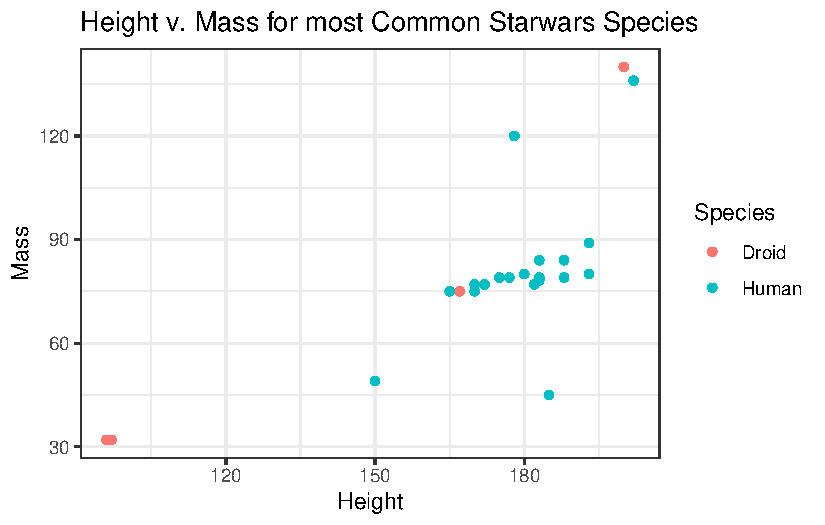
\includegraphics{thesis_draft_files/figure-pdf/example-figure-1.pdf}

}

\caption{Example Figure Title/Caption}

\end{figure}

\hypertarget{how-to-add-tables}{%
\section{How to Add Tables}\label{how-to-add-tables}}

\begin{longtable}[]{@{}lrr@{}}
\caption{Example Table Title/Caption }\tabularnewline
\toprule()
name & height & mass \\
\midrule()
\endfirsthead
\toprule()
name & height & mass \\
\midrule()
\endhead
Luke Skywalker & 172 & 77 \\
C-3PO & 167 & 75 \\
R2-D2 & 96 & 32 \\
\bottomrule()
\end{longtable}

\hypertarget{conclusion}{%
\chapter{Conclusion}\label{conclusion}}

Write something here I guess.

\hypertarget{computational-details}{%
\section{Computational Details}\label{computational-details}}

The results in this paper were obtained using \texttt{R} 4.4.1.
\texttt{R} itself and all packages used are available from the
Comprehensive \texttt{R} Archive Network (CRAN) at
https://CRAN.R-project.org/.

\hypertarget{references}{%
\chapter*{REFERENCES}\label{references}}
\addcontentsline{toc}{chapter}{REFERENCES}

\hypertarget{refs}{}
\begin{CSLReferences}{1}{0}
\leavevmode\vadjust pre{\hypertarget{ref-r_core_team_r_2024}{}}%
R Core Team. (2024). \emph{R: {A} {Language} and {Environment} for
{Statistical} {Computing}}. Vienna, Austria: R Foundation for
Statistical Computing. Retrieved from \url{https://www.R-project.org/}

\end{CSLReferences}

\appendix

\let\oldclearpage\clearpage
\let\oldcleardoublepage\cleardoublepage

\let\clearpage\relax
\let\cleardoublepage\relax

\hypertarget{super-cool-fancy-function}{%
\chapter{Super Cool Fancy Function}\label{super-cool-fancy-function}}

\let\clearpage\oldclearpage
\let\cleardoublepage\oldcleardoublepage

\begin{Shaded}
\begin{Highlighting}[]
\CommentTok{\# Add your fancy function here!}
\end{Highlighting}
\end{Shaded}

\hypertarget{slightly-less-cool-fancy-something}{%
\chapter{Slightly Less Cool Fancy
Something}\label{slightly-less-cool-fancy-something}}

\begin{Shaded}
\begin{Highlighting}[]
\CommentTok{\# Got more fancy functions, or figures, or tables, }
\CommentTok{\# or pretty much anything?}
\end{Highlighting}
\end{Shaded}




\end{document}
